\documentclass[chi_draft]{sigchi}

% Use this section to set the ACM copyright statement (e.g. for
% preprints).  Consult the conference website for the camera-ready
% copyright statement.

% Copyright
\CopyrightYear{2018}
%\setcopyright{acmcopyright}
\setcopyright{acmlicensed}
%\setcopyright{rightsretained}
%\setcopyright{usgov}
%\setcopyright{usgovmixed}
%\setcopyright{cagov}
%\setcopyright{cagovmixed}
% DOI
\doi{http://dx.doi.org/10.475/123_4}
% ISBN
\isbn{123-4567-24-567/08/06}
%Conference
\conferenceinfo{ASSETS'18,}{October 22--24, 2018, Galway, Ireland}
%Price
\acmPrice{\$15.00}

% Use this command to override the default ACM copyright statement
% (e.g. for preprints).  Consult the conference website for the
% camera-ready copyright statement.

%% HOW TO OVERRIDE THE DEFAULT COPYRIGHT STRIP --
%% Please note you need to make sure the copy for your specific
%% license is used here!
% \toappear{
% Permission to make digital or hard copies of all or part of this work
% for personal or classroom use is granted without fee provided that
% copies are not made or distributed for profit or commercial advantage
% and that copies bear this notice and the full citation on the first
% page. Copyrights for components of this work owned by others than ACM
% must be honored. Abstracting with credit is permitted. To copy
% otherwise, or republish, to post on servers or to redistribute to
% lists, requires prior specific permission and/or a fee. Request
% permissions from \href{mailto:Permissions@acm.org}{Permissions@acm.org}. \\
% \emph{CHI '16},  May 07--12, 2016, San Jose, CA, USA \\
% ACM xxx-x-xxxx-xxxx-x/xx/xx\ldots \$15.00 \\
% DOI: \url{http://dx.doi.org/xx.xxxx/xxxxxxx.xxxxxxx}
% }

% Arabic page numbers for submission.  Remove this line to eliminate
% page numbers for the camera ready copy
% \pagenumbering{arabic}

% Load basic packages
\usepackage{balance}       % to better equalize the last page
\usepackage{graphics}      % for EPS, load graphicx instead 
\usepackage[T1]{fontenc}   % for umlauts and other diaeresis
\usepackage{txfonts}
\usepackage{mathptmx}
\usepackage[pdflang={en-US},pdftex]{hyperref}
\usepackage{color}
\usepackage{xspace}
\usepackage{booktabs}
\usepackage{textcomp}

% Some optional stuff you might like/need.
\usepackage{microtype}        % Improved Tracking and Kerning
% \usepackage[all]{hypcap}    % Fixes bug in hyperref caption linking
\usepackage{ccicons}          % Cite your images correctly!
% \usepackage[utf8]{inputenc} % for a UTF8 editor only

% If you want to use todo notes, marginpars etc. during creation of
% your draft document, you have to enable the "chi_draft" option for
% the document class. To do this, change the very first line to:
% "\documentclass[chi_draft]{sigchi}". You can then place todo notes
% by using the "\todo{...}"  command. Make sure to disable the draft
% option again before submitting your final document.
\usepackage{todonotes}

% Paper metadata (use plain text, for PDF inclusion and later
% re-using, if desired).  Use \emtpyauthor when submitting for review
% so you remain anonymous.
\def\plaintitle{Leveraging Augmented Reality to Create Orientation and Mobility Apps for People with Visual Disabilities}
\def\plainauthor{First Author, Second Author, Third Author,
  Fourth Author, Fifth Author, Sixth Author}
\def\emptyauthor{}
\def\plainkeywords{orientation and mobility; augmented reality; assistive tech}
\def\plaingeneralterms{Documentation, Standardization}

% llt: Define a global style for URLs, rather that the default one
\makeatletter
\def\url@leostyle{%
  \@ifundefined{selectfont}{
    \def\UrlFont{\sf}
  }{
    \def\UrlFont{\small\bf\ttfamily}
  }}
\makeatother
\urlstyle{leo}

% To make various LaTeX processors do the right thing with page size.
\def\pprw{8.5in}
\def\pprh{11in}
\special{papersize=\pprw,\pprh}
\setlength{\paperwidth}{\pprw}
\setlength{\paperheight}{\pprh}
\setlength{\pdfpagewidth}{\pprw}
\setlength{\pdfpageheight}{\pprh}

% Make sure hyperref comes last of your loaded packages, to give it a
% fighting chance of not being over-written, since its job is to
% redefine many LaTeX commands.
\definecolor{linkColor}{RGB}{6,125,233}
\hypersetup{%
  pdftitle={\plaintitle},
% Use \plainauthor for final version.
%  pdfauthor={\plainauthor},
  pdfauthor={\emptyauthor},
  pdfkeywords={\plainkeywords},
  pdfdisplaydoctitle=true, % For Accessibility
  bookmarksnumbered,
  pdfstartview={FitH},
  colorlinks,
  citecolor=black,
  filecolor=black,
  linkcolor=black,
  urlcolor=linkColor,
  breaklinks=true,
  hypertexnames=false
}


\newcommand{\BVI}{B/VI\xspace}
\newcommand{\OM}{O\&M\xspace}

% create a shortcut to typeset table headings
% \newcommand\tabhead[1]{\small\textbf{#1}}

% End of preamble. Here it comes the document.
\begin{document}

\title{\plaintitle}

\numberofauthors{3}
\author{%
  \alignauthor{Leave Authors Anonymous\\
    \affaddr{for Submission}\\
    \affaddr{City, Country}\\
    \email{e-mail address}}\\
  \alignauthor{Leave Authors Anonymous\\
    \affaddr{for Submission}\\
    \affaddr{City, Country}\\
    \email{e-mail address}}\\
  \alignauthor{Leave Authors Anonymous\\
    \affaddr{for Submission}\\
    \affaddr{City, Country}\\
    \email{e-mail address}}\\
}

\maketitle

\begin{abstract}
The introduction of augmented reality technology to iOS and Android enables, for the first time, mainstream smartphones to estimate their own motion in 3D space with high accuracy.  For assistive technology researchers, this development presents an enormous opportunity.  In this spirit, we present our work leveraging these technologies to create two smartphone apps to empower people with visual disabilities to more easily perform orientation and mobility tasks.  Our first app provides automatic navigation guidance when backtracking along a route.  Our second app utilizes crowdsourcing to provide automatic guidance to objects of interest.  We present the design of these apps along with a usability study.  Our work expands the capabilities of assistive technology for orientation and mobility that can be distributed cheaply at massive scale.  We conclude by discussing the opportunities, pitfalls, and limitations of augmented reality for creating orientation and mobility apps.
\end{abstract}

\category{K.4.2.}{Assistive technology for persons with disabilities}{Orientation and mobility tools for persons with visual disabilities}

\keywords{\plainkeywords}

\section{Introduction}
For people who are blind or visually impaired (\BVI), improvements in orientation and mobility (\OM) have been shown to increase economic opportunity as well as psychological well-being.  For instance, while only 30\% of working-age Americans who are \BVI are employed \cite{employmentstatistics2017, kirchner1999looking}, individuals with better \OM skills fare better at finding employment \cite{crudden1998comprehensive, crudden1999barriers, leonard1999factors, o1999employment}.  Due to the importance of \OM, there is a long history of assistive technology designed to bolster these skills  \cite{benjamin1973new, borenstein1997guidecane}.  Despite considerable effort, historically, few of these technologies have achieved much impact beyond the lab \cite{wiener2010foundations}.  This lack of impact has been driven, largely, by the fact that the technologies were either expensive, unreliable, cumbersome, did not provide significant benefits over simpler solutions, or were hard to distribute at mass scale.

Major exceptions to this disappointing track record are GPS navigation apps for smartphones.  Since these apps are mainstream technologies that happen to be universally accessible --- as opposed to special purpose assistive technologies --- they are highly robust, powerful, and extremely useful to people who are \BVI.  Further, the fact that a majority of people who are \BVI own smartphones \cite{morris2014blind} makes them distributable at either no additional cost (e.g., Google Maps) or at modest cost (e.g., BlindSquare which is designed for people who are \BVI and costs about \$30).

While being incredibly useful, GPS apps for \OM have major shortcomings.  Most notably, GPSes in modern smartphones are only accurate to about $5m$ under open sky (and are even worse in challenging environments such as cities) and do not work indoors.  Researchers are working to build systems that overcome these challenges (see \emph{Related Work}).

Recently, smartphone manufacturers have introduced augmented reality modules (AR), which support high accuracy 3D-tracking.  While the primary purpose of these modules is to enable AR applications --- whereby virtual and real content are mingled, e.g., by overlaying virtual characters on a smartphone's camera feed --- these modules have the potential to be repurposed to create assistive technology for \OM that is highly robust, accurate, usable, widely deployable, and free.

With the significant potential of smartphone-based AR technology come critical research questions.  Are the motion estimates provided by AR robust enough to use for \OM, and, if so, which \OM tasks might be facilitated?  In this document we begin to provide answers to these questions.  Specifically, we present our work utilizing user-centered design to leverage the AR modules in modern smartphones to create assistive technologies to aid users who are \BVI with \OM tasks.%  In order to design maximally impactful technologies, we employ user-centered design principles throughout our research and development process.%  Specifically, we worked longitudinally with co-designers who are \BVI and two of the study authors, who are visually impaired themselves, contributed to all aspects of the project and provided design guidance based on their personal experiences.

Our first app, \emph{Clew}, enables users to backtrack along previously traveled routes.  \emph{Clew} is designed to alleviate various pain points experienced by non-visual travelers (e.g., finding one's way independently after being led to a location by a sighted guide).  The second app, \emph{ViewShare}, utilizes crowdsourcing to enable a user to find objects in cluttered environments.  In the remainder of the paper we present related work on \OM assistive technology, discuss the algorithms that underlie AR technology on modern smartphones, present the design of \emph{Clew} and \emph{ViewShare}, provide preliminary usability data for \emph{Clew}, and finally conclude with a discussion of future challenges and promising directions for smartphone-based AR technology for people who are \BVI.

\section{Related work}

A number of researchers have worked to overcome the limitations (e.g., less-than-ideal accuracy, lack of availability indoors) of GPS technology for assisting people who are \BVI with \OM.  Researchers have pursued roughly two approaches.  The first is to utilize crowdsourcing, whereby people who are \BVI connect over the internet with a sighted person for realtime assistance.  Examples of this approach include the VizWiz project \cite{bigham2010vizwiz}, BeMyEyes \cite{bemyeyesaccessworld}, and Aira \cite{aira} (both BeMyEyes and Aira support a video chat interface).  A second approach combines rudimentary motion estimates derived from inertial sensors (gyroscopes and accelerometers) with detection of fixed environmental infrastructure (e.g., Bluetooth beacons, Wifi access points).  For instance, \cite{ganz2015percept, ganz2011percept, ganz2014percept} developed a system for navigation using smartphone-detectable RFID tags.  Dias and her collaborators utilized WiFi fingerprinting and dead-reckoning for indoor navigation \cite{Dias__2014_7778}, and similar systems based on Bluetooth beacons have also been developed \cite{ishihara2017beacon, ahmetovic2016navcog}.  Others have explored the use of robots, with sophisticated sensors, to act as guides for people who are blind \cite{Nanavati:2018:CIN:3173386.3176976}.

Another area of research is the development of solutions to help people who are \BVI find objects that were misplaced, moved by a third party, or whose locations were never known.  While the task of object finding doesn't fall under the umbrella of \OM, here we stretch the terminology to encompass it by noting that both \OM and object finding require a significant degree of spatial awareness.  As in the case of navigation, crowdsourcing approaches have shown promise for object finding \cite{bigham2010vizwizlocateit}.  Other approaches use automatic object detection and tracking to navigate to objects \cite{schauerte2012assistive, jafri2014computer, thakoor2014system}.%\todo{might need to explicitly contrast with our work, why is ours better, or just say that we will discuss this later}

\section{Augmented Reality}
%
%\begin{figure}
%\begin{center}
%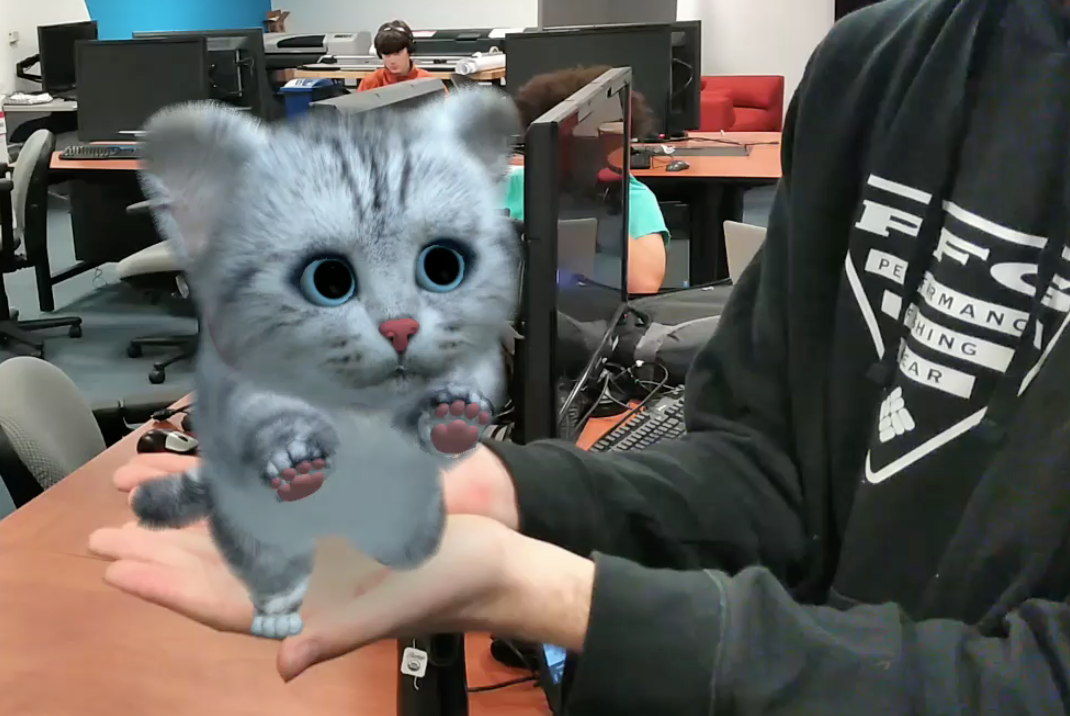
\includegraphics[width=.9\linewidth]{Figures/arexample.png}
%\end{center}
%\caption{A virtual cat overlaid on a smartphone camera feed.  The phone is able to accurately sense its movement in order to render the cat at the appropriate viewing angle and depth.\label{fig:arexample}}
%\end{figure}

Recently, both Apple and Google have released support for highly sophisticated smartphone-based AR experiences, whereby virtual and real content are combined.  For instance, an app might show a virtual cat projected into a real world scene.  As the user moves, the phone senses the user's motion and renders the cat at an appropriate distance and angle, providing the illusion that the cat exists in the physical world.

These AR systems utilize 3D motion-processing algorithms that are vastly more accurate than the inertial-based systems in previous \OM apps.  The high accuracy of these systems is driven by two key trends: the development of sophisticated algorithms for visual-inertial odometry (VIO) \cite{li2013high,leutenegger2015keyframe,bloesch2015robust,forster2014svo} (which combine optical tracking with inertial sensing to perform motion estimation) and the development of special purpose hardware that allows these computationally intensive algorithms to run with minimal heat generation and power consumption.  It is the combination of high accuracy and low power consumption that has the potential to unlock many new potential \OM apps for people who are \BVI.

\subsection{Algorithms for Visual Inertial Odometry}
While a full explanation of VIO \cite{gui2015review} is beyond the scope of this paper, it helps to have a conceptual understanding of VIO.  VIO algorithms are designed for either the monocular (single camera) or stereo setting.  Since the monocular setting is the one applicable to mass-market smartphones, here we use the term VIO to refer to monocular VIO specifically.

VIO algorithms utilize sensor fusion to blend optical and inertial motion estimates.  Optical motion estimates are made by tracking salient visual features --- e.g., corners or other highly textured portions of an image --- through multiple video frames.  Utilizing the mathematics of perspective geometry, one can estimate the rotation and translation of the phone \cite{Hartley2004}.  Importantly, the accuracy of these estimates is dependent on tracking a large number of visual features that should, ideally, correspond to points at a range of depths from the camera.%  While some environments are intrinsically more difficult for optical tracking, we have observed that users may exacerbate this difficulty by holding their phones in a suboptimal orientation (e.g., with the camera facing the ground).

Further complicating matters, the translation estimated using optical tracking is only determined up to an arbitrary scale factor.  This indeterminacy arises due to the fact that the depths of the tracked visual features are unknown \cite{Hartley2004}.  For example, given an estimate of the translation of the phone, it is possible that the phone moved twice as far and the depths of the tracked points were twice as great.  The shortcomings of optical tracking, scale-indeterminacy and inaccurate performance in feature-poor environments, can be overcome by the fusion of inertial data (gyroscopes and accelerometers).  Gyroscopes, which provide accurate estimates of angular velocity, can refine estimates of rotation while accelerometer data can be integrated over time to obtain estimates of linear velocity, overcoming the scale-indeterminacy problem.%  Since inertial sensors don't function optimally when subjected to fast rotations or high accelerations, users should hold their phones relatively stable for maximum accuracy.

\subsection{VIO in Mass-Market Smartphones}
Both Apple and Google have released AR modules based on VIO.  While, the details of their VIO algorithms are not publicly available, there are distinctions between these frameworks that researchers should keep in mind.

\subsubsection{Google Tango}
Release in late 2014 by Google's ATAP (Advanced Technology and Projects) division, the Tango utilizes a wide-angle lens and a global image shutter to enable accurate visual-feature tracking.  The platform also includes a PrimeSense depth-sensing camera.  Two commercial smartphones have been released based on the Tango platform: the Lenovo Phab2 Pro and the Asus Zenfone AR.  While the tracking capabilities of Tango devices are superior to both ARKit and ARCore (discussed next), the reliance on special-purpose hardware has severely limited the adoption of the technology.  As a result, Google suspended the project in early 2018 \cite{tangoretired}.


\subsubsection{ARKit and ARCore}

Apple's ARKit \cite{arkit} and Google's ARCore \cite{arcore}, both released in 2017, do not require special purpose hardware.  Since these platforms utilize conventional cameras, the richness of visual features available for tracking is not as great as with Tango, and consequently, their motion estimates are less accurate.  Further, since neither of these platforms have depth sensing cameras, the availability of 3D information is limited to objects with special structure (e.g., planar horizontal and vertical surfaces).  Despite their drawbacks, these frameworks can run on a wider share of phones than Google Tango, however, given the large preference for iOS among people who are \BVI \cite{morris2014blind}, ARKit is the primary platform of interest for researchers seeking to develop \OM apps for people who are \BVI.

%Although quite specific and certainly at the implementation detail level, a challenge presented when developing assistive apps for ARKit is that the ARSCNView class provided by Apple does not allow for the presentation of subviews.  This limitation makes it particular hard to achieve optimal integration with Apple's VoiceOver.  In particular, it is very difficult to make an app that consistently announces the identity of activated buttons, while also properly announcing new controls that appears on the screen.

\section{Design Process and Insights}
We employed semi-structured interviews, participatory design approaches \cite{buhler2001empowered, schuler1993participatory}, and digital prototype testing over a period of a month with members of the \BVI community.  We engaged deeply with one co-designer named Joe (name changed for anonymous review), a college student who has no functional vision due to Retinitis Pigmentosa (a degenerative vision disorder that leads to the breakdown of cells in the retina); he is a non-visual traveler, mostly navigating with the help of his guide dog. We also learned from an \OM trainer for primary and middle school students who shared stories drawn from his own experiences. Furthermore, two members of our research team, who are themselves visually impaired, contributed both to the design and implementation of the apps and leveraged their personal experiences and knowledge of the \BVI community to inform our design process. Our research team identified a number of pain points and accessibility barriers through involving people who work with or identify as \BVI people throughout aspects of our design and evaluation.

\textbf{Navigating newly traveled routes towards previously visited locations was difficult.} Joe expressed that finding his seat (e.g., in a classroom) after going to the restroom was challenging, particularly when traveling without his dog. This story resonated for one of our visually impaired team members who found it difficult to find his seat on a dimly lit airplane while returning from the restroom. These insights motivated the creation of our app \emph{Clew} to support precise indoor navigation for finding the way back in unfamiliar environments.

\textbf{Finding objects in unfamiliar environments was difficult.} While Joe mentioned he had no difficulty in finding objects in spaces he has control to organize himself, he admitted that locating objects of interest in unfamiliar places or when others disturb his organization can be very challenging. Additionally, finding precise locations in outdoor environments (e.g., the correct part of a train platform or button to activate a crosswalk) is very difficult.  This set of insights helped support the creation of our app \emph{ViewShare} for object finding.

Over the course of our multi-week co-design with Joe, he tried various prototypes as a means to explore potential concepts for assistive apps.  Based on his feedback, we developed a mostly complete version of \emph{Clew}, which he was able to test and help us to improve.  While informed by his insights, Joe did not test \emph{ViewShare} as it was developed after he had returned to college.

\section{App 1: Clew}


\begin{figure}
\begin{center}
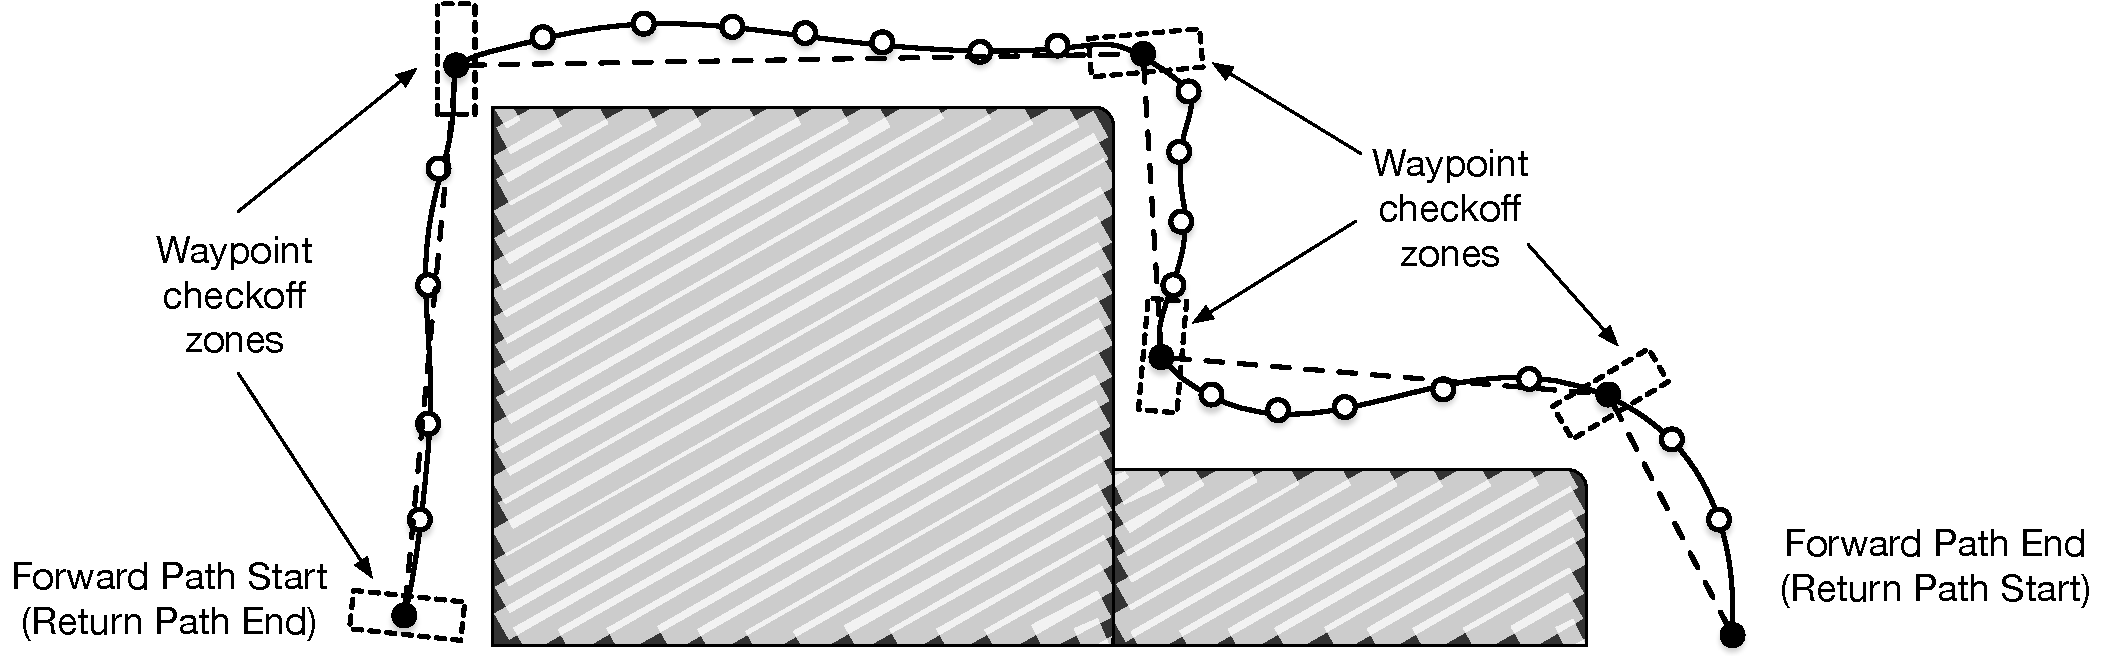
\includegraphics[width=\linewidth]{Figures/samplepath}
\end{center}
\caption{A topdown view of a path generated by the \emph{Clew}.  The figure shows the raw path (solid line) and breadcrumbs (white circles with black outlines).  The Ramer-Douglas-Peucker reduces the breadcrumbs to a more manageable number of waypoints (solid black circles).  The resultant path consists of straight lines connecting these waypoints in reverse order.  Waypoint checkoff zones are shown as dashed boxes).\label{fig:samplepath}}
\end{figure}

We present \emph{Clew}, an iPhone app based on ARKit (link to Clew on the app store redacted).  Clew provides turn-by-turn directions to guide users who are \BVI along previously traveled routes.  The app has two primary use cases.  First, when a user is led somewhere by a sighted guide, they may wish to return to their previous location at a later time --- without wanting to be guided back.  Secondly, sometimes it is easier for someone who is \BVI to navigate from a location than back to it.  For instance, it is easier for someone who is \BVI to leave a conference room than it is to find their way back to their particular seat.  For both of these uses cases, \emph{Clew} provides high-accuracy, easy-to-follow, navigational guidance to enable people who are \BVI to travel independently indoors, without the need for modifications to the environment (e.g., the introduction of beacons or special signage).  

Clew works by dropping a trail of virtual breadcrumbs (representing timestamped 3D positions), which can be followed in reverse order at a later time.  The phase of laying down these breadcrumbs is called \emph{path recording} mode.  In \emph{path recording} mode, the user holds their smartphone with the screen facing towards them and the camera facing roughly parallel to the ground.  The user then travels to a new location (either via their traditional \OM process or via assistance from a sighted guide) and stops the recording.  Figure~\ref{fig:samplepath} shows a sample path along with virtual breadcrumbs.%  A virtual breadcrumb (shown as a white circle with a black outline) is dropped at a fixed time interval.
%
%\begin{figure}
%\begin{center}
%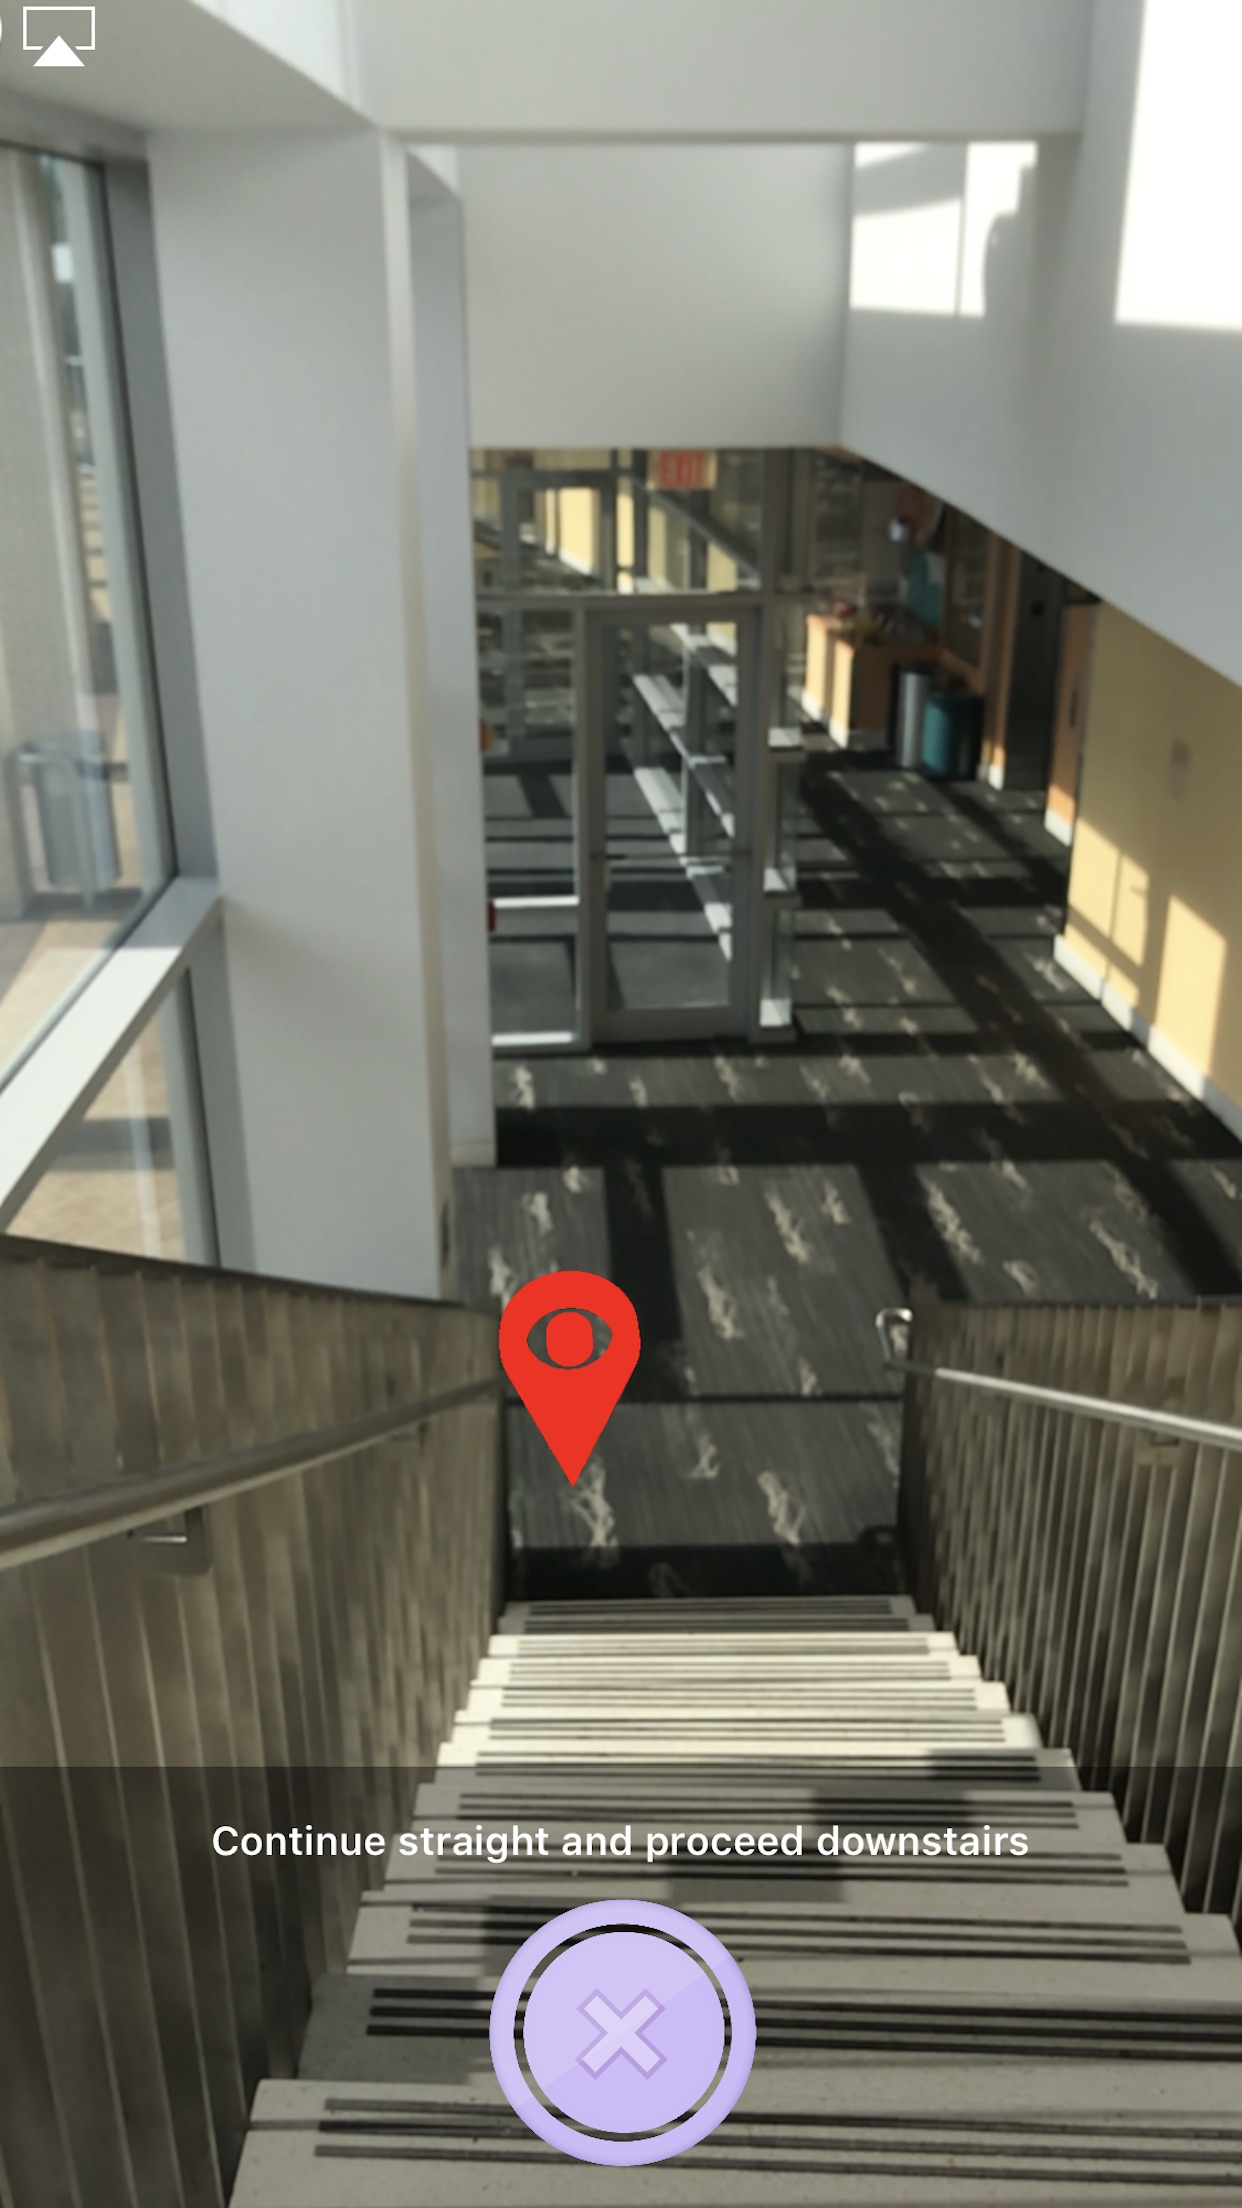
\includegraphics[width=0.48\linewidth]{Figures/clew_screenshot_1}\hspace{.01\linewidth}
%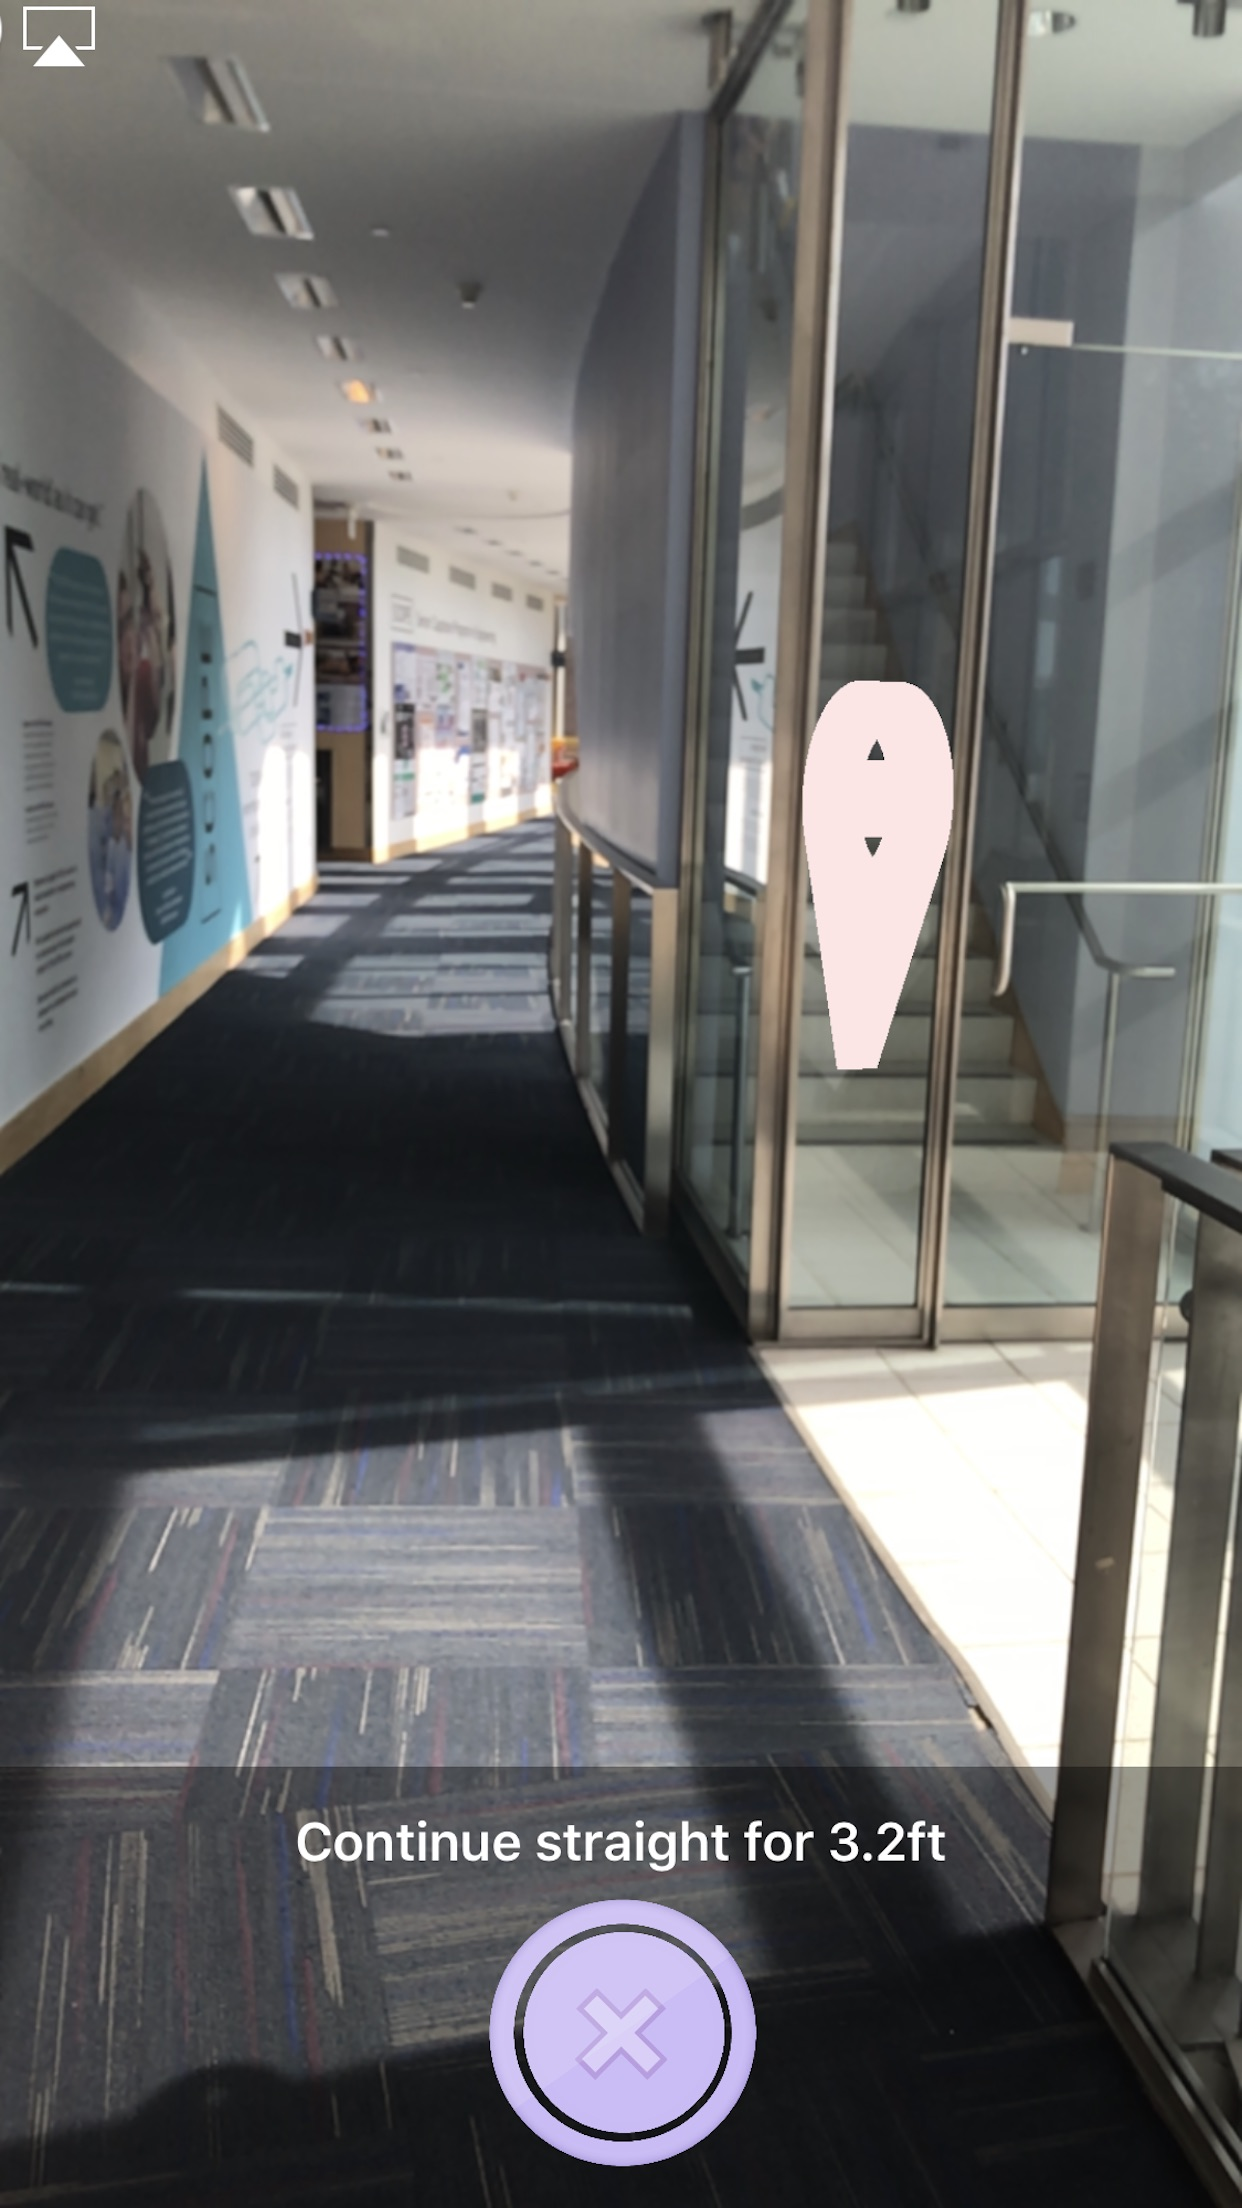
\includegraphics[width=0.48\linewidth]{Figures/clew_screenshot_2}
%\end{center}
%\caption{Two screenshots from our app ``Clew'' in navigation mode (where a user is retracing a previously traveled route).  The text for the left image says ``Continue straight and proceed downstairs'' and the text on the right says ``Continue straight for 3.2 feet.''\label{fig:clewshots}}
%\end{figure}

When the user has recorded their path, they can either pause (described later) or navigate back along their route.  When navigating back, the trail of breadcrumbs is processed by the Douglas-Ramer-Peucker (DPR) algorithm \cite{douglas1973algorithms} for path simplification.  This algorithm winnows down the path by removing sequences of breadcrumbs that are well represented by a straight line.  Figure~\ref{fig:samplepath} shows the breadcrumbs selected by the DPR algorithm, called \emph{waypoints}, and the resultant piecewise straight navigation route obtained by connecting the waypoints.  In \emph{navigation mode}, the app synthesizes directions to the next waypoint using one of three mechanisms: (1) speech (e.g., ``continue straight for 10 feet''), (2) haptic or (3) audible feedback when the phone is pointing towards the next waypoint.  When using (2) or (3), the low latency of the update of the phone's position allows the user to sweep their phone back and forth until they sense a haptic or auditory cue, providing an accurate sense of the direction to the next waypoint.

As the user navigates, the app continuously checks to see if the user has reached the next waypoint.  We define the condition of ``reached the next waypoint'' as the user entering a \emph{waypoint checkoff zone} (see Figure~\ref{fig:samplepath}).  Instead of making these checkoff zones spherical, we made them rectangular prisms with sides perpendicular to the direction of travel longer than for dimensions parallel to the direction of travel.  This choice of shape enables the user to deviate laterally from the intended path without missing a waypoint.  The app also announces flights of stairs by detecting if the vertical angle of the segment connecting two waypoints exceeds a threshold.

\subsection{Pause feature}
While an ARKit tracking session is running, the user must not switch to a different app, lock the phone, or occlude the camera.  This can be a hindrance when the user wants to wait a significant amount of time before navigating back, when the user would like to use another app, or when the user needs both of their hands to perform some task.  ARKit does support a pause feature for a tracking session, however, when the session is resumed the phone's position will remain the same as before it was paused.  Given this limitation, we designed a pause feature that prompts the user to place their phone in a position and orientation (collectively called a ``pose'') that is easy to return to when the user wants to resume.  It is not crucial that the user be able to perfectly recreate this pose.  Specifically, the most important aspect of the pose to recreate is its yaw.  The reason for this is that the phone's accelerometer can easily determine the other two degrees of freedom of rotation (as these are not perpendicular to gravity) and deviations in the phone's position cause a fixed amount of error, whereas an error in the phone's yaw will be magnified the farther the user travels.  Holding the phone's screen flat against features such as walls or doors works well for this purpose.  

\subsection{Novelty in Relationship to Previous Work}
Our work on the design of \emph{Clew} represents the first research into automatically guiding a user back along a route, without the need for special modifications to the environment.
\subsection{Usability Testing}

\begin{table}
  \centering
  \begin{tabular}{l r r r | r  r}
    % \toprule
    {\small \textit{Length}}
      & {\small \textit{Stairs}}
    & {\small \textit{Visuals}}
        & {\small \textit{Success}}
        & {\small \textit{Mean Error}} 
                & {\small \textit{Median Error}} \\
    \midrule
    21.3m & no & good & 100\% & 0.15m & 0.15m \\
    40.2m & yes & mixed & 100\% & 0.99m & 0.91m \\
    11.9m & no & poor & 100\% & 0.91m & 0.61m \\
    22.9m & no & good & 100\% & 1.45m & 1.37m \\
        47.2m & yes & mixed & 100\%& 1.45m & 1.37m \\
            43.4m & yes & good & 75\% & 2.03m & 1.83m \\
    % \bottomrule
  \end{tabular}
  \caption{Usability results for Clew.  The \emph{Visuals} column indicates the availability of trackable visual features, with ``mixed'' indicating that a route had segments with both good and poor quality visual features.}~\label{tab:clewusability}
\end{table}

As a preliminary usability test, four college students used Clew to navigate six routes.  For each route, the participant was led by one of the authors --- mimicking the role of a sighted guide --- and then navigated back using Clew.  Participants were instructed to follow the guidance of the app, avoiding the use of their memory to correct for the app's errors.  In order to become accustomed to the app, the participants were sighted for the first two trial routes.  A trial was unsuccessful if the user couldn't follow the app's guidance (e.g., the app's estimation of a waypoint's location was inside a wall due to a failure of the ARKit's tracking algorithm). For successful trials (the user navigated to all waypoints), we recorded the distance from the user's final position to the ground truth position.  A summary of each of the routes and the results are shown in Table~\ref{tab:clewusability}.  These results demonstrate the robustness of Clew for navigating fairly complex routes, including routes that navigate stairs and/or through places with poor visual features.  The current study, while promising, is limited by its use of participants with occluded vision, rather than people who are \BVI.  While our co-designer who is blind tested Clew extensively, we are currently working on a full evaluation of Clew with multiple users who are \BVI.

\subsection{Future Work for Clew}
First, in order to make \emph{Clew} successful, we must continue to engage deeply with users to understand how they experience the current version of the app and improve it based on their feedback. Second, we are working to improve the ability of the app to detect and communicate tracking failures.  Specifically, when ARKit throws an error, it is straightforward to communicate this information to the user; however, if tracking drifts or becomes inaccurate without throwing an error, detection is much more difficult. Third, we are working to enable the sharing of previously traveled routes with other users.  This feature will work similarly to the pause feature in that the user will place their phone in a known starting pose (e.g., against a door as they enter a building), allowing their phone to register its current pose with the starting pose of a saved route.

\section{App 2: ViewShare}

Finding objects in unfamiliar environments can be challenging for people who are \BVI.  Inspired by previous work \cite{bigham2010vizwizlocateit} that utilizes a crowdsourcing model, whereby sighted online volunteers label an object of interest and sonic cues automatically guide a user to an object, we developed the \emph{ViewShare} app.

\emph{ViewShare} provides high precision, automatic guidance to objects of interest.  To begin, the user, who is \BVI, launches the ViewShare app, starting an ARKit tracking session.  When the user wants to find an object, they announce its name, the phone recognizes their voice command, and a localization job is created.  This job is assigned to multiple sighted volunteers, who are sent push notifications on their smartphones.  On the \BVI user's device, every two seconds a snapshot of their environment is captured and added to the job.  Once a volunteer clicks on the push notification they are shown the snapshots (see Figure~\ref{fig:viewsharescreenshots}).  After the volunteer locates the object, they tap its position on the screen.  The object location in the image, represented as a 2D pixel coordinate, is relayed back to the \BVI user's app, which then attempts to convert this coordinate into a 3D position (see \emph{2D to 3D Transformation}).  If a 3D location can be determined, the user is provided with automatic guidance to the object in the form of computer-generated speech and haptic feedback.

\subsection{Object Localization Feedback}
ViewShare communicates location information using haptic and speech feedback.  Specifically, whenever the phone is oriented towards a located object the phone will vibrate subtly and the distance and name of the object will be announced.  To facilitate finding objects in 3D, the app provides two localization modes.  In \emph{2D feedback mode} the distance and orientation to an object are determined by projecting 3D spatial information into the floor plane.  This mode is useful for navigating to objects that are far away (since the height of the object is irrelevant until the user gets closer).  In \emph{3D feedback mode} distances and orientations to objects are determined using the unmodified 3D information.  This mode is useful for finding objects that are nearby.%  As an example, 3D mode is suited to finding a pen and 2D mode is suited to finding a door.

\begin{figure}
\begin{center}
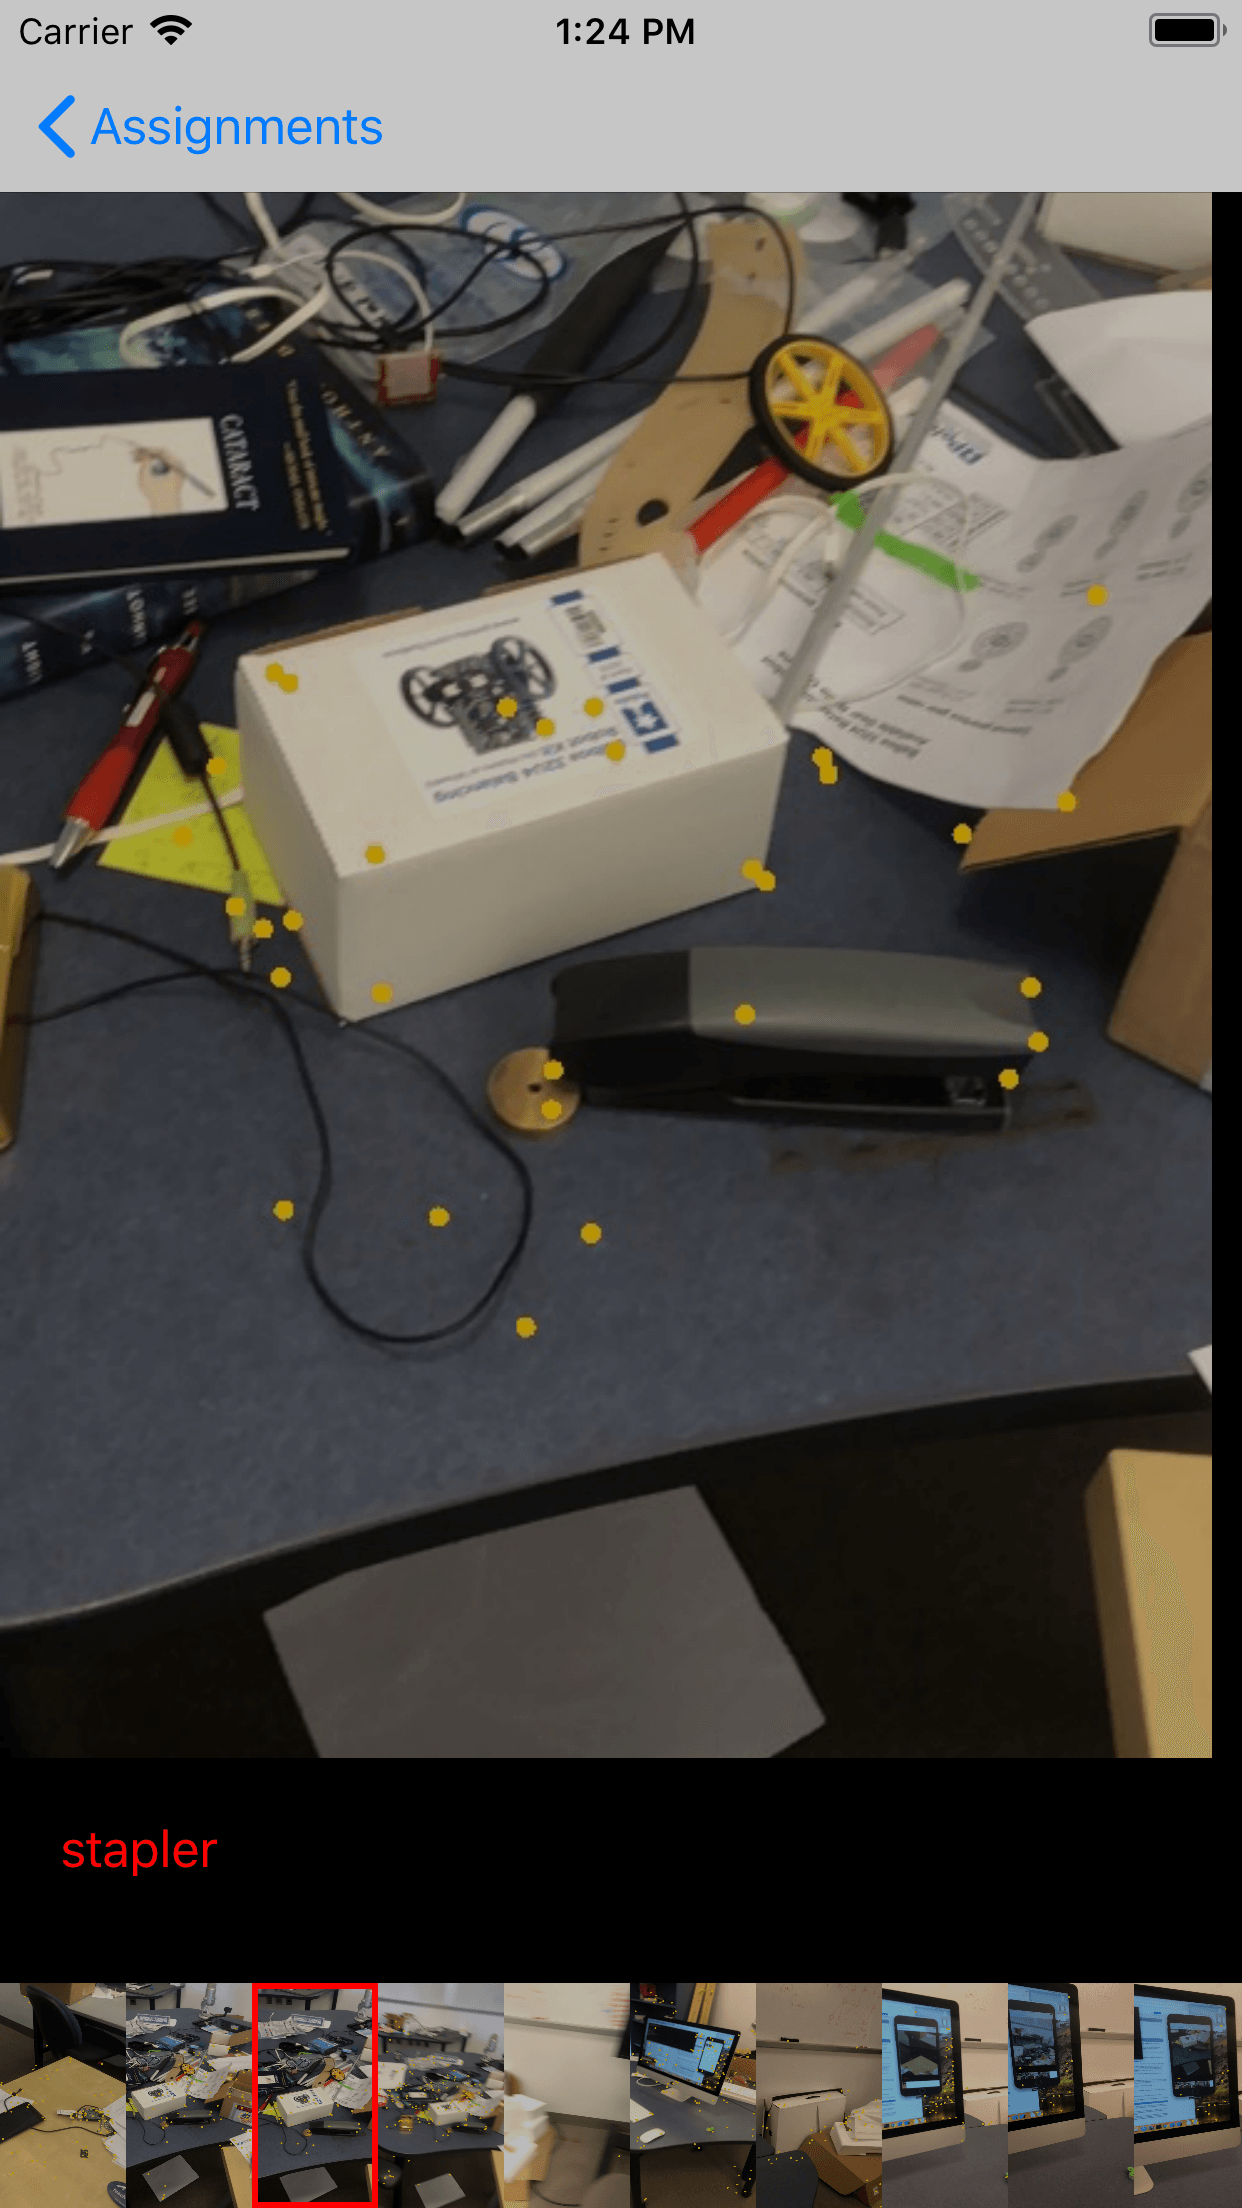
\includegraphics[height=3in]{Figures/viewshare_crowdworker}\hspace{.01\linewidth}
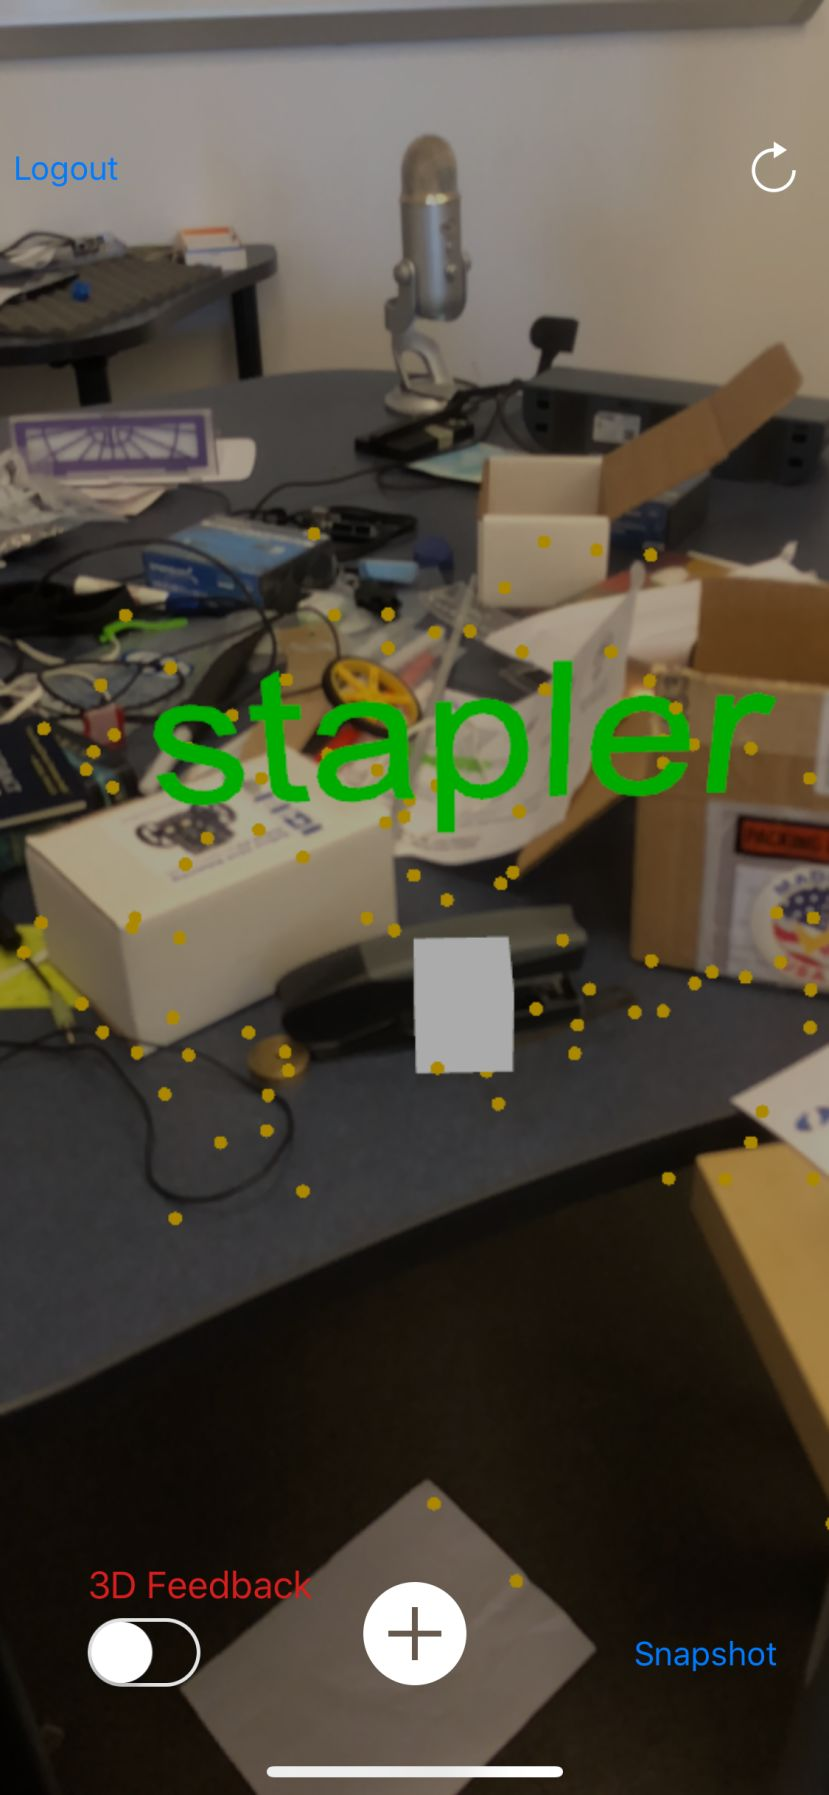
\includegraphics[height=3in]{Figures/viewshare_user}
\end{center}
\caption{Left: ViewShare's interface for the crowdworker.  The crowdworker is instructed to locate the stapler in the images collected from the \BVI user's phone.  \textbf{Right:} the interface for the \BVI user showing the location of the stapler as indicated by the crowdworker (the visualization is useful primarily for users with low vision and as a debugging tool).\label{fig:viewsharescreenshots}}
\end{figure}


\subsection{2D to 3D Transformation}
In order to map a 2D pixel coordinate to a 3D point in space, we utilize ARKit's plane fitting feature.  We first test whether the ray that connects the optical center of the camera with the location of the pixel coordinate of the located object intersects a tracked 3D plane (ARKit is capable of finding both vertical and horizontal planes in 3D).  If the ray intersects a plane, we mark the object as localized and compute its 3D position using standard geometric formulas.  If the ray \emph{does not} intersect a known plane (either because the object is not located on a plane or because the plane has not been found by ARKit) we return an error condition.  In this situation, the volunteer is instructed to click on the object from a second viewpoint.  Once the 2D pixel coordinate of the object is provided in two views, we use triangulation to compute its 3D position. % The optimal 3D triangulation of two rays with endpoints $x_1$ and $x_2$ and unit directions $u_1$ and $u_2$ is given by the following equation.
%
%\begin{align}
%%c&= x_2 - x_1 \nonumber \\
%%D &= x_1 + u_1 \frac{\left ( u_2 u_2^\top u_1  +  u_1   \right )^\top \left ( x_2 - x_1 \right) } {1 - \left ( u_1^\top u_2 \right)^2} \nonumber \\
%%E &= x_2 + u_2 \frac{ \left ( u_1 u_2^\top u_1 - u_2 \right )^\top  \left ( x_2 - x_1 \right)  }{1 -  \left ( u_1^\top u_2 \right)^2} \nonumber \\
%&\mbox{triangulate}(x_1, u_1, x_2, u_2) \nonumber = \\
%&\frac{x_1 + x_2}{2}  + \frac{ u_1 u_1^\top u_2 u_2^\top  +  u_1 u_1^\top  + u_2 u_1^\top  u_2 u_1^\top - u_2 u_2^\top }{2 \left (1 -  \left ( u_1^\top u_2 \right)^2\right) } \left(  x_2 - x_1\right) \nonumber
%\end{align}
%

%
%        let A = ray1.origin
%        let B = ray2.origin
%        let a = ray1.direction
%        let b = ray2.direction
%        let c = B - A
%        let D = A + a*(-simd_dot(a,b)*simd_dot(b,c)+simd_dot(a,c)*simd_dot(b,b))/(simd_dot(a,a)*simd_dot(b,b) - simd_dot(a,b)*simd_dot(a,b))
%        let E = B + b*(simd_dot(a,b)*simd_dot(a,c)-simd_dot(b,c)*simd_dot(a,a))/(simd_dot(a,a)*simd_dot(b,b) - simd_dot(a,b)*simd_dot(a,b))
%        let closestPoint = (D + E)/2

\subsection{Novelty in Relationship to Previous Work}
Our work on \emph{ViewShare} represents the first development of an app designed specifically for object finding that leverages the built-in motion sensing capabilities to both localize and provide guidance to objects in 3D.  Previous approaches either use a more brittle, 2D, approach to object localization, or require imprecise, mentally taxing, and high latency verbal communication to relay location information.

\subsection{Future Work for ViewShare}
While we designed this app primarily for finding objects, it can be utilized for other tasks.  One possibility is finding things that are not objects (e.g., the precise location of a bus stop or a doorway in outdoor settings where GPS is not sufficiently accurate).  A second possibility is automatically providing the location of important features in the environment (e.g., doors, windows, chairs) so that the user can make a mental map of the space around them.  In addition to these new use cases, another area of future exploration is quality control.  Aggregating judgments from multiple workers is an active area of research and these techniques can be utilized to filter inaccurate localizations from the crowd.

\section{Discussion and Future Directions}

\subsection{Robustness of AR motion estimates for precise \OM} Our study demonstrates that for navigation routes of $\sim45m$ the motion estimates of ARKit are sufficiently accurate.  Additionally, for object finding within a room or on a tabletop we have found, anecdotally, that ARKit's performance is sufficient.

As the complexity of the environment increases other sources of information (e.g., the detection of landmarks such as optical tags or Bluetooth beacons) could reduce tracking drift, providing spatial anchors.  Alternatively, crowdsourcing could correct drift in the phone's motion estimates (e.g., a crowdworker might identify a landmark at two points in time).

\subsection{Usability Concerns of \OM technology using AR}
Since AR relies on VIO, which leverages optical tracking, apps based on AR require the camera to be unoccluded.  Currently, our apps assume that the user holds their phone in one hand while holding their cane in the other.  Future research should consider whether a method of handsfree operation can be developed that allows the user to continue to use their phone as an interface.  This could work by using an attachment (e.g., a neck lanyard) for holding the phone coupled with a speech-based user interface.  We are currently exploring this idea.

For apps that require the user to hold the phone in their hand, recall that VIO algorithms work best when they are able to detect a large number of visual features at a range of depths.  This condition is best achieved when the user holds their phone upright with the camera facing approximately parallel to the ground.  We found that Joe had difficulty maintaining the phone in this configuration, perhaps due to the lack of visual feedback about the phone's orientation.  As a result, tracking performance suffered.  Developers of AR-powered assistive apps should consider adding feedback mechanisms to help the user to maintain their phone in an optimal orientation. 
\balance{}

\section{Conclusion}
We have presented two smartphone apps that allow people who are \BVI to perform difficult \OM tasks with their smartphones.  Our apps are among the first mass-distributable apps for navigation and object finding in unmodified indoor environments.  While the results of our usability study are promising, more work, particularly in concert with users who are \BVI, is required to further refine the developed apps.

Additionally, we have outlined several promising areas of opportunity for the development of AR apps for \OM and provided a discussion of the usability factors of this technology.  Through the development of new algorithms, co-design with users, and the improvement of AR technology itself, researchers can hopefully continue to leverage AR to create impactful smartphone technology for people who are \BVI.  
%
%\section{Acknowledgments}
%Removed for anonymous review.

% BALANCE COLUMNS

\newpage
% REFERENCES FORMAT
% References must be the same font size as other body text.
\bibliographystyle{SIGCHI-Reference-Format}
\bibliography{../references/assets,../references/assistive_tech,../references/disability_studies,../references/machine_learning}

\end{document}

%%% Local Variables:
%%% mode: latex
%%% TeX-master: t
%%% End:
